\documentclass[zihao=-4,a4paper,fontset=windows]{ctexart}
% ---------- 版心：左侧留出密封线位置 ----------
\usepackage[a4paper,left=4.85cm,right=0.95cm,top=2.3cm,bottom=2.4cm,headsep=0.4cm,footskip=0.9cm]{geometry}
\usepackage{amsmath,amssymb}
% ---------- 字体：Times New Roman + 宋体/黑体，与 HIT 试卷一致 ----------
\setmainfont{Times New Roman}
\usepackage{newtxmath}
\usepackage{bm}
\setCJKmainfont[AutoFakeBold=2.5]{SimSun}
\setCJKsansfont{SimHei}
\newCJKfontfamily\stliti{STLiti}
\linespread{1.08}\selectfont

\usepackage{enumitem}
\usepackage{booktabs,array,multirow}
\usepackage{tikz}
\usetikzlibrary{positioning,arrows.meta,calc}
\usepackage{fancyhdr}
\usepackage{lastpage}
\usepackage{xcolor}
\usepackage{needspace}

% ---------- 页眉页脚 ----------
\newcommand{\coursename}{模式识别与机器学习A}
\newcommand{\pagefoot}{\zihao{5}\textbf{第\thepage 页（共\pageref{LastPage}页）}}
\pagestyle{fancy}
\fancyhf{}
\fancyhead[C]{\zihao{-5}\coursename}
\renewcommand{\headrulewidth}{0.4pt}
\renewcommand{\footrulewidth}{0.6pt}
\fancyfoot[R]{\pagefoot}
\fancyfootoffset[L]{2.35cm}
\fancypagestyle{firstpage}{%
  \fancyhf{}\renewcommand{\headrulewidth}{0pt}%
  \renewcommand{\footrulewidth}{0.6pt}\fancyfoot[R]{\pagefoot}\fancyfootoffset[L]{2.35cm}}

% ---------- 常用命令 ----------
\setlist{itemsep=1pt,topsep=2pt,parsep=0pt}
\setlist[enumerate,1]{leftmargin=2.2em}
% 选择题选项：\opts 两列排布（短选项），\optss 每项一行（长选项）
\newcommand{\opts}[4]{\par\nopagebreak\noindent\hspace*{1.5em}%
  \begin{tabular}{@{}p{0.45\linewidth}p{0.45\linewidth}@{}}A. #1 & B. #2\\ C. #3 & D. #4\end{tabular}\par}
\newcommand{\optss}[4]{\par\nopagebreak\noindent\hspace*{1.5em}%
  \begin{tabular}{@{}p{0.92\linewidth}@{}}A. #1\\ B. #2\\ C. #3\\ D. #4\end{tabular}\par}
\newcommand{\blank}[1][2.5cm]{\underline{\hspace{#1}}}
\newcommand{\judge}{（\hspace{1.5em}）}
\newcommand{\pts}[1]{（#1分）}
\newcommand{\sect}[1]{\par\needspace{5\baselineskip}\medskip\noindent{\zihao{4}\heiti #1}\par\smallskip}
\newcommand{\ans}[1]{\textcolor{blue!60!black}{#1}}
\DeclareMathOperator*{\argmax}{arg\,max}
\DeclareMathOperator*{\argmin}{arg\,min}
\newcommand{\E}{\mathbb{E}}
\newcommand{\KL}{D_{\mathrm{KL}}}
\newcommand{\pending}[1]{{\zihao{5}［#1］}}
\newcommand{\recallnote}[1]{\par\nopagebreak\noindent\pending{#1}\par}
\newcommand{\problem}[1]{\par\addvspace{\medskipamount}\needspace{4\baselineskip}\noindent\textbf{#1}\par\nopagebreak}

\begin{document}

\thispagestyle{firstpage}
% ===== 卷头：仿哈工大试卷，按页面绝对坐标定位（单位 cm，原点为页面左上角，y 向下） =====
\noindent\begin{tikzpicture}[remember picture,overlay,x=1cm,y=-1cm,shift={(current page.north west)}]
  % 主管领导审核签字栏
  \draw[line width=0.6pt] (3.6,1.6) rectangle (4.8,8.3);
  \draw[line width=0.6pt] (3.6,4.2) -- (4.8,4.2);
  \node[align=center,font=\zihao{-4}\songti,inner sep=0pt] at (4.2,2.9)
    {主管\\[-2pt]领导\\[-2pt]审核\\[-2pt]签字};
  % 标题
  \node[font=\zihao{-2}\heiti] at (11.6,1.95) {哈尔滨工业大学 2026 年秋季学期};
  \node[font=\zihao{2}\heiti] at (12.6,3.35) {模式识别与机器学习（A）\hspace{0.45em}试题（回忆版）};
  % 题号 / 得分 / 阅卷人（3 行，13 列）
  \def\xs{5.2,6.55,7.67,8.79,9.91,11.03,12.15,13.27,14.39,15.51,16.63,17.75,18.87,20.05}
  \foreach \y in {4.90,5.98,7.06,8.14} \draw[line width=0.5pt] (5.2,\y) -- (20.05,\y);
  \foreach \x in \xs \draw[line width=0.5pt] (\x,4.90) -- (\x,8.14);
  \foreach \t/\xa/\xb in {题号/5.2/6.55,一/6.55/7.67,二/7.67/8.79,
      三.1/8.79/9.91,三.2/9.91/11.03,三.3/11.03/12.15,三.4/12.15/13.27,三.5/13.27/14.39,
      三.6/14.39/15.51,三.7/15.51/16.63,三.8/16.63/17.75,三.9/17.75/18.87,总分/18.87/20.05}
    \node[font=\zihao{-4}\heiti] at ({(\xa+\xb)/2},5.44) {\t};
  \node[font=\zihao{-4}\heiti] at (5.875,6.52) {得分};
  \node[font=\zihao{-4}\heiti] at (5.875,7.60) {阅卷人};
  % 片纸鉴心 诚信不败
  \node[font=\fontsize{26pt}{30pt}\selectfont\stliti] at (11.6,9.05) {片纸鉴心\hspace{0.6em}诚信不败};
  \draw[line width=0.6pt] (2.5,9.75) -- (3.3,9.75);
  \draw[line width=0.6pt] (4.6,9.75) -- (20.05,9.75);
  % 密封线（内侧，带“密”“封”）
  \draw[densely dotted,line width=1pt] (4.5,9.2) -- (4.5,27.0);
  \foreach \y/\t in {15.6/密,21.3/封}
    \node[fill=white,inner sep=1.5pt,font=\zihao{-4}\songti] at (4.32,\y) {\t};
  % 学生信息（外侧，竖排）
  \draw[densely dotted,line width=1pt] (3.95,9.2) -- (3.95,27.0);
  \foreach \yb/\t/\len in {13.9/授课教师/2.8,17.9/姓名/3.0,22.0/学号/3.1,26.6/院系/3.4}
    \node[rotate=90,anchor=west,fill=white,inner xsep=2pt,font=\zihao{-4}\heiti] at (3.1,\yb)
      {\t\rule[-1.5pt]{\len cm}{0.5pt}};
\end{tikzpicture}%
\vspace*{6.85cm}

\noindent{\zihao{5}本卷据 2026 年 11 月 22 日考后口述和同学补充整理。方括号内为回忆提示或待核对的内容。}

\sect{一、单项选择题（共 5 题）}
\begin{enumerate}[label=\arabic*.]
\item \judge 关于验证集和测试集的选择题。 \pending{题干与选项待补。}
\item \judge 下列哪一项属于回归任务的评价指标？
\optss{召回率、精确率和 \(F_1\)}{均方误差（MSE）和平均绝对误差（MAE）}{混淆矩阵}{ROC 曲线下的面积（AUC）}
\item \judge 下列哪些任务不需要对数据进行标注？
\par\nopagebreak\noindent （1） 用 K-means 对客户分组\quad （2） \pending{一项需要标注的任务}
\par\nopagebreak\noindent （3） 医疗图像去噪\quad （4） 涉及 GMM 的任务\quad （5） \pending{待补}
\opts{\pending{组合待补}}{\pending{组合待补}}{\pending{组合待补}}{\pending{组合待补}}
\recallnote{编号暂排。去噪任务可能提到 VAE。}
\item \judge 关于支持向量机（SVM）的选择题。 \pending{题干原句待核对。}
\optss{硬间隔 SVM 要求训练数据线性可分。}{涉及软间隔 SVM 的效果。 \pending{完整表述待补。}}{\pending{待补。}}{SVM 只能用于多分类，不能用于二分类。}
\item \judge 题目与贝叶斯方法及数据集标注有关。 \pending{题干原句待补。}
\par\nopagebreak\noindent （1）\ \blank[0.7cm]\quad （2）\ \blank[0.7cm]\quad （3）\ \blank[0.7cm]\quad
（4）\ \blank[0.7cm]\quad （5）\ \blank[0.7cm]\quad \pending{条目待补}
\opts{\pending{组合待补}}{\pending{组合待补}}{\pending{组合待补}}{\pending{组合待补}}
\end{enumerate}

\sect{二、判断对错题（共 10 题，在题前括号内打“√”或“×”）}
\noindent\pending{第 2、3、8 题暂排，第 4 题暂按同学回忆定位。朴素贝叶斯和模型评估两题相邻，暂列第 5、6 题。}
\begin{enumerate}[label=\arabic*.]
\item \judge 有关 EM 算法的 E 步、M 步与极大似然估计的关系。 \pending{原判断句措辞待核对。}
\item \judge 单层感知机不能解决异或问题，叠加多个单层感知机也不能解决。 \pending{题干是否指定激活函数等条件待核对。}
\item \judge 逻辑回归模型对预测概率设置阈值后，可以用于分类。
\item \judge HMM 的齐次马尔可夫性意味着当前隐状态依赖此前的全部隐状态。 \pending{题干还提到观测独立性假设，原句待核对。}
\item \judge 朴素贝叶斯分类器中的“朴素”指各特征之间相互独立。 \pending{原题是否写明“给定类别”待核对。}
\item \judge 类别不均衡时，仅凭准确率评价分类模型可能不够，还应参考 \(F_1\)、召回率等指标。 \pending{口述记作“精确度”，原题的指标名称待核对。}
\item \judge LSTM 从结构上可以输出整个输入序列的全部信息，Transformer 不能并行计算。 \pending{原句措辞待核对。}
\item \judge Transformer 只能使用可学习的嵌入，不能使用固定的正弦或余弦。 \pending{原题说的是词嵌入还是位置编码待核对。}
\item \judge 最大池化和平均池化是否含有可学习参数。 \pending{原判断句的肯定或否定措辞待核对。}
\item \judge CNN 卷积层的不同卷积核之间共享参数。
\end{enumerate}

\sect{三、计算与分析题（共 9 题）}

\problem{1. 卷积与最大池化}
给定一个 \(5\times5\) 的输入矩阵。
\begin{enumerate}[label=(\arabic*)]
\item 用卷积核 \(K=\begin{pmatrix}1&2\\0&1\end{pmatrix}\)、偏置 \(b=1\) 计算卷积输出。
\item 对卷积输出做最大池化，池化窗口为 \(2\times2\)，步长为 \(1\)。
\end{enumerate}
\pending{输入矩阵、卷积步长和填充待补。卷积核按口述“1201”逐行排列。}

\problem{2. 逻辑回归}
写出逻辑回归的模型结构和 sigmoid 函数。设权重 \(\bm w=(2,-1)^\top\)，偏置 \(b=1\)，对样本 \(\bm x_1=(1,2)^\top\) 和 \(\bm x_2=(-2,-1)^\top\) 完成计算。 \pending{所要求的具体量待补，可能是 \(P(y=1\mid\bm x)\)。}

\problem{3. 支持向量机的软间隔}
\begin{enumerate}[label=(\arabic*)]
\item 解释什么是线性可分、什么是线性不可分。
\item 说明软间隔是怎样引入的，并解释松弛变量 \(\xi_i\) 的含义。
\end{enumerate}

\problem{4. 循环神经网络}
下图是含两层隐藏层的 RNN 沿时间展开的结构，隐藏层激活函数为 \(\tanh\)。写出从输入 \(\bm x_t\) 经隐藏状态 \(\bm h_t^{1}\)、\(\bm h_t^{2}\) 到输出 \(\bm o_t\) 的完整计算过程（偏置等符号自行定义）。
\begin{center}
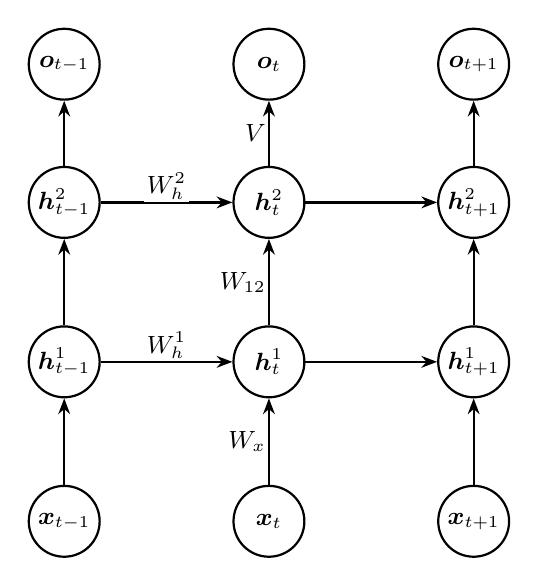
\begin{tikzpicture}[x=2.6cm,y=1.35cm,>={Stealth[length=2mm]},
    nd/.style={circle,draw,thick,minimum size=9mm,inner sep=0pt,font=\small},
    lb/.style={font=\small,fill=white,inner sep=1pt}]
  \foreach \i/\t in {0/t-1,1/t,2/t+1}{
    \node[nd] (x\i) at (\i,0) {\(\bm x_{\t}\)};
    \node[nd] (a\i) at (\i,1.5) {\(\bm h^{1}_{\t}\)};
    \node[nd] (b\i) at (\i,3) {\(\bm h^{2}_{\t}\)};
    \node[nd] (o\i) at (\i,4.3) {\(\bm o_{\t}\)};
    \draw[->,thick] (x\i) -- (a\i);
    \draw[->,thick] (a\i) -- (b\i);
    \draw[->,thick] (b\i) -- (o\i);}
  \foreach \i/\j in {0/1,1/2}{
    \draw[->,thick] (a\i) -- (a\j);
    \draw[->,thick] (b\i) -- (b\j);}
  \node[lb,left]  at ($(x1)!0.5!(a1)$) {\(W_x\)};
  \node[lb,left]  at ($(a1)!0.5!(b1)$) {\(W_{12}\)};
  \node[lb,left]  at ($(b1)!0.5!(o1)$) {\(V\)};
  \node[lb,above] at ($(a0)!0.5!(a1)$) {\(W_h^{1}\)};
  \node[lb,above] at ($(b0)!0.5!(b1)$) {\(W_h^{2}\)};
\end{tikzpicture}
\end{center}
\pending{据考后手绘图重画。原图未标第二层隐藏层的循环权重，图中记作 \(W_h^{2}\)；输出层是否接 softmax 待核对。}

\problem{5. 删除非支持向量}
删去非支持向量后，重新求得的分离超平面会不会改变？说明理由。

\problem{6. 学习率与训练误差}
\begin{enumerate}[label=(\arabic*)]
\item 为什么学习率过大会使训练过程出现震荡？应如何调整？
\item 调整学习率后，训练误差仍然较大。写出两个可能原因。
\end{enumerate}

\problem{7. 交叉熵与 KL 散度}
给定概率分布 \(P=(0.50,\,0.25,\,0.25)\) 和 \(Q=(1,\,0,\,0)\)。
\begin{enumerate}[label=(\arabic*)]
\item 计算 \(P\) 与 \(Q\) 的交叉熵。 \pending{交叉熵的参数顺序待核对。}
\item 设分布 \(R\) 与 \(P\) 完全相同，计算 KL 散度 \(D_{\mathrm{KL}}(R\|P)\)。
\end{enumerate}

\problem{8. 贝叶斯分类器}
简述贝叶斯分类器的基本原理。说明先验概率、后验概率和类条件概率分别指什么。

\problem{9. 多项式回归与过拟合}
\begin{enumerate}[label=(\arabic*)]
\item 给定模型 \(\hat y=0.5x^2-1\) 及两个样本 \((x,y)=(3,\,3.2)\) 和 \((4,\,7.5)\)，计算均方误差 MSE。
\item 选用的多项式阶数过高可能出现什么现象？写出两种缓解方法。
\end{enumerate}

\end{document}
